\chapter{ORIUS Architecture: DC3S Runtime Layer}
\label{ch:orius-architecture-dc3s}

ORIUS enters the dissertation at the narrowest and most consequential point in the control
loop: after nominal intelligence has proposed an action, but before that action is allowed
to alter a physical plant. That placement is deliberate. Batteries, vehicles, industrial
systems, healthcare monitors, navigation stacks, and aerospace controllers do not share one
estimator, one optimizer, or one plant model. What they can share is a disciplined runtime
treatment of what happens when degraded observation changes the meaning of safe release.

\section{Why a runtime layer is the right object}
The architectural claim is therefore narrower and stronger than a proposal for a universal
controller. Degraded observation creates a release-boundary problem that sits between
inference and actuation. Once telemetry becomes stale, delayed, missing, or corrupted, the
relevant question is no longer only ``what would the nominal controller do?'' It becomes
``what action can still be justified for physical release under the observation quality now
available?'' ORIUS is the layer that answers that second question.

That framing is what lets the book stay universal without drifting into abstraction. The
runtime layer leaves domain-specific controllers, estimators, and plant models in place
while freezing one common control-flow grammar for degraded observation. That grammar is
Detect, Calibrate, Constrain, Shield, and Certify.

\section{The DC3S release step}
The universal runtime step has five stages.
\begin{description}
  \item[Detect] compute observation reliability from freshness, missingness, delay,
  ordering, spikes, and consistency markers;
  \item[Calibrate] widen the observation-consistent state set as reliability falls;
  \item[Constrain] recompute the admissible action set under the widened uncertainty set;
  \item[Shield] repair the candidate action or replace it with a bounded fallback when no
  admissible repaired action remains;
  \item[Certify] emit a causal certificate describing the reliability state, uncertainty
  summary, repaired action, fallback status, and lifecycle metadata that govern release.
\end{description}

What matters is not that each stage is unprecedented in isolation. The architectural move is
the typed composition of all five at one runtime boundary. ORIUS treats degraded observation
as something that must change release semantics immediately, not as a warning signal that
can be logged while nominal actuation proceeds unchanged.

\section{Universal runtime flow}
\begin{figure}[htbp]
\centering
\IfFileExists{reports/publication/fig_orius_theory_runtime_domain_flow.png}{%
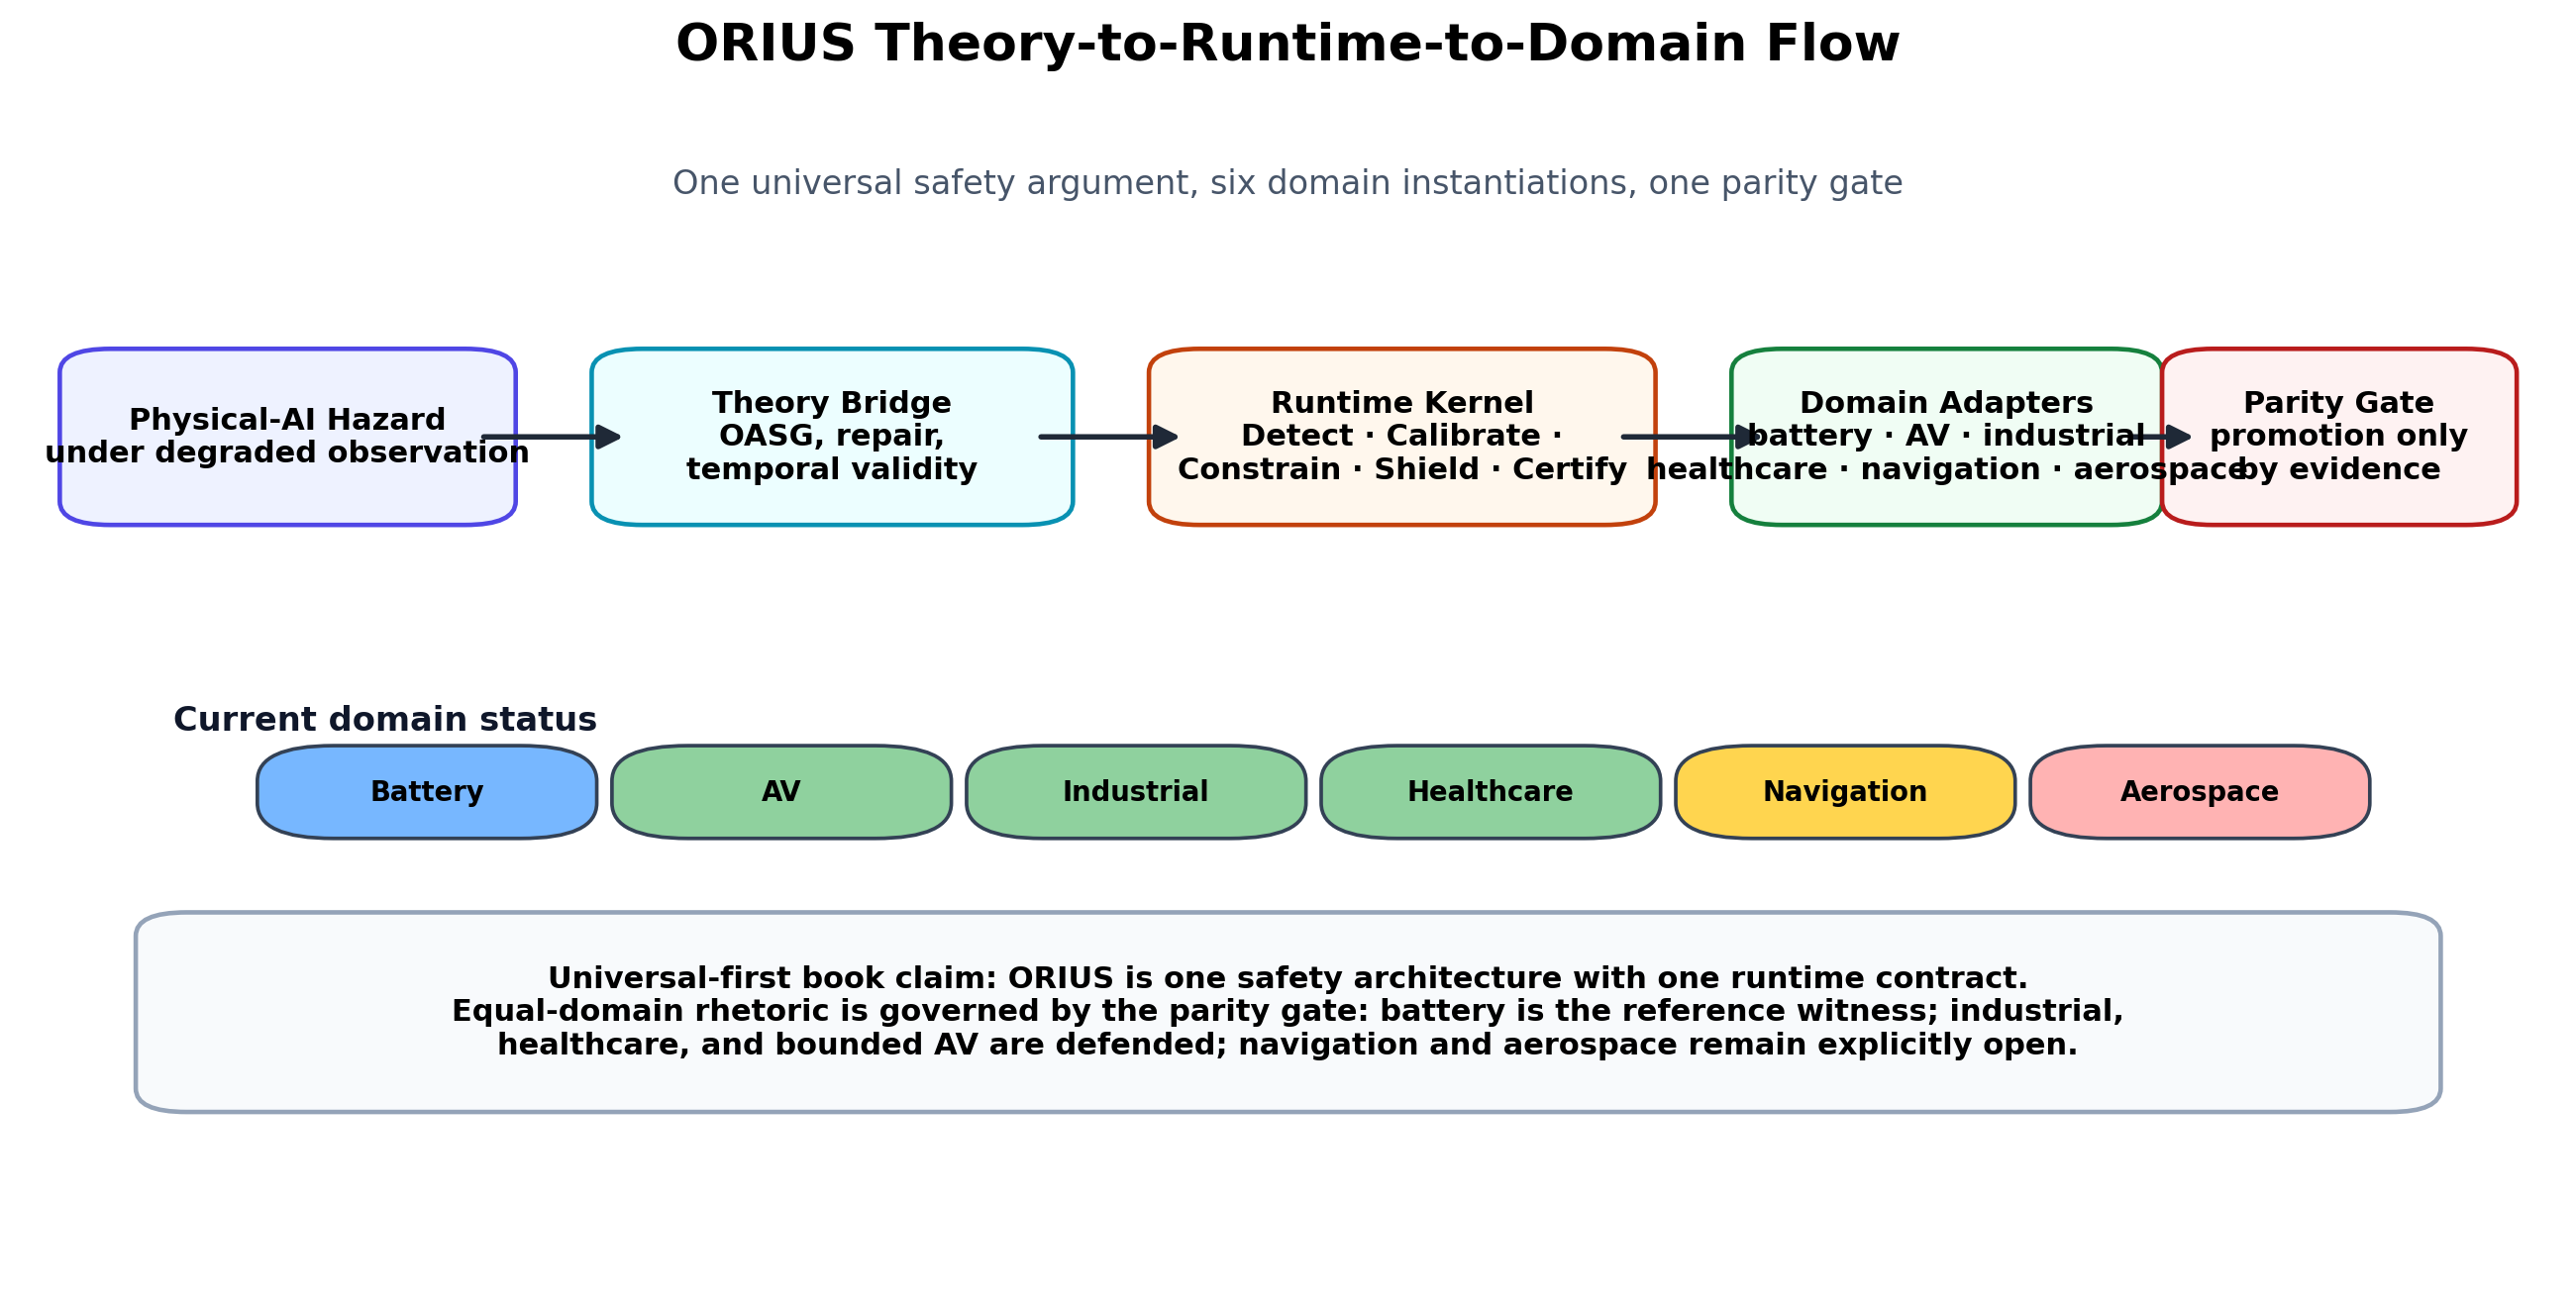
\includegraphics[width=0.94\textwidth]{reports/publication/fig_orius_theory_runtime_domain_flow.png}%
}{%
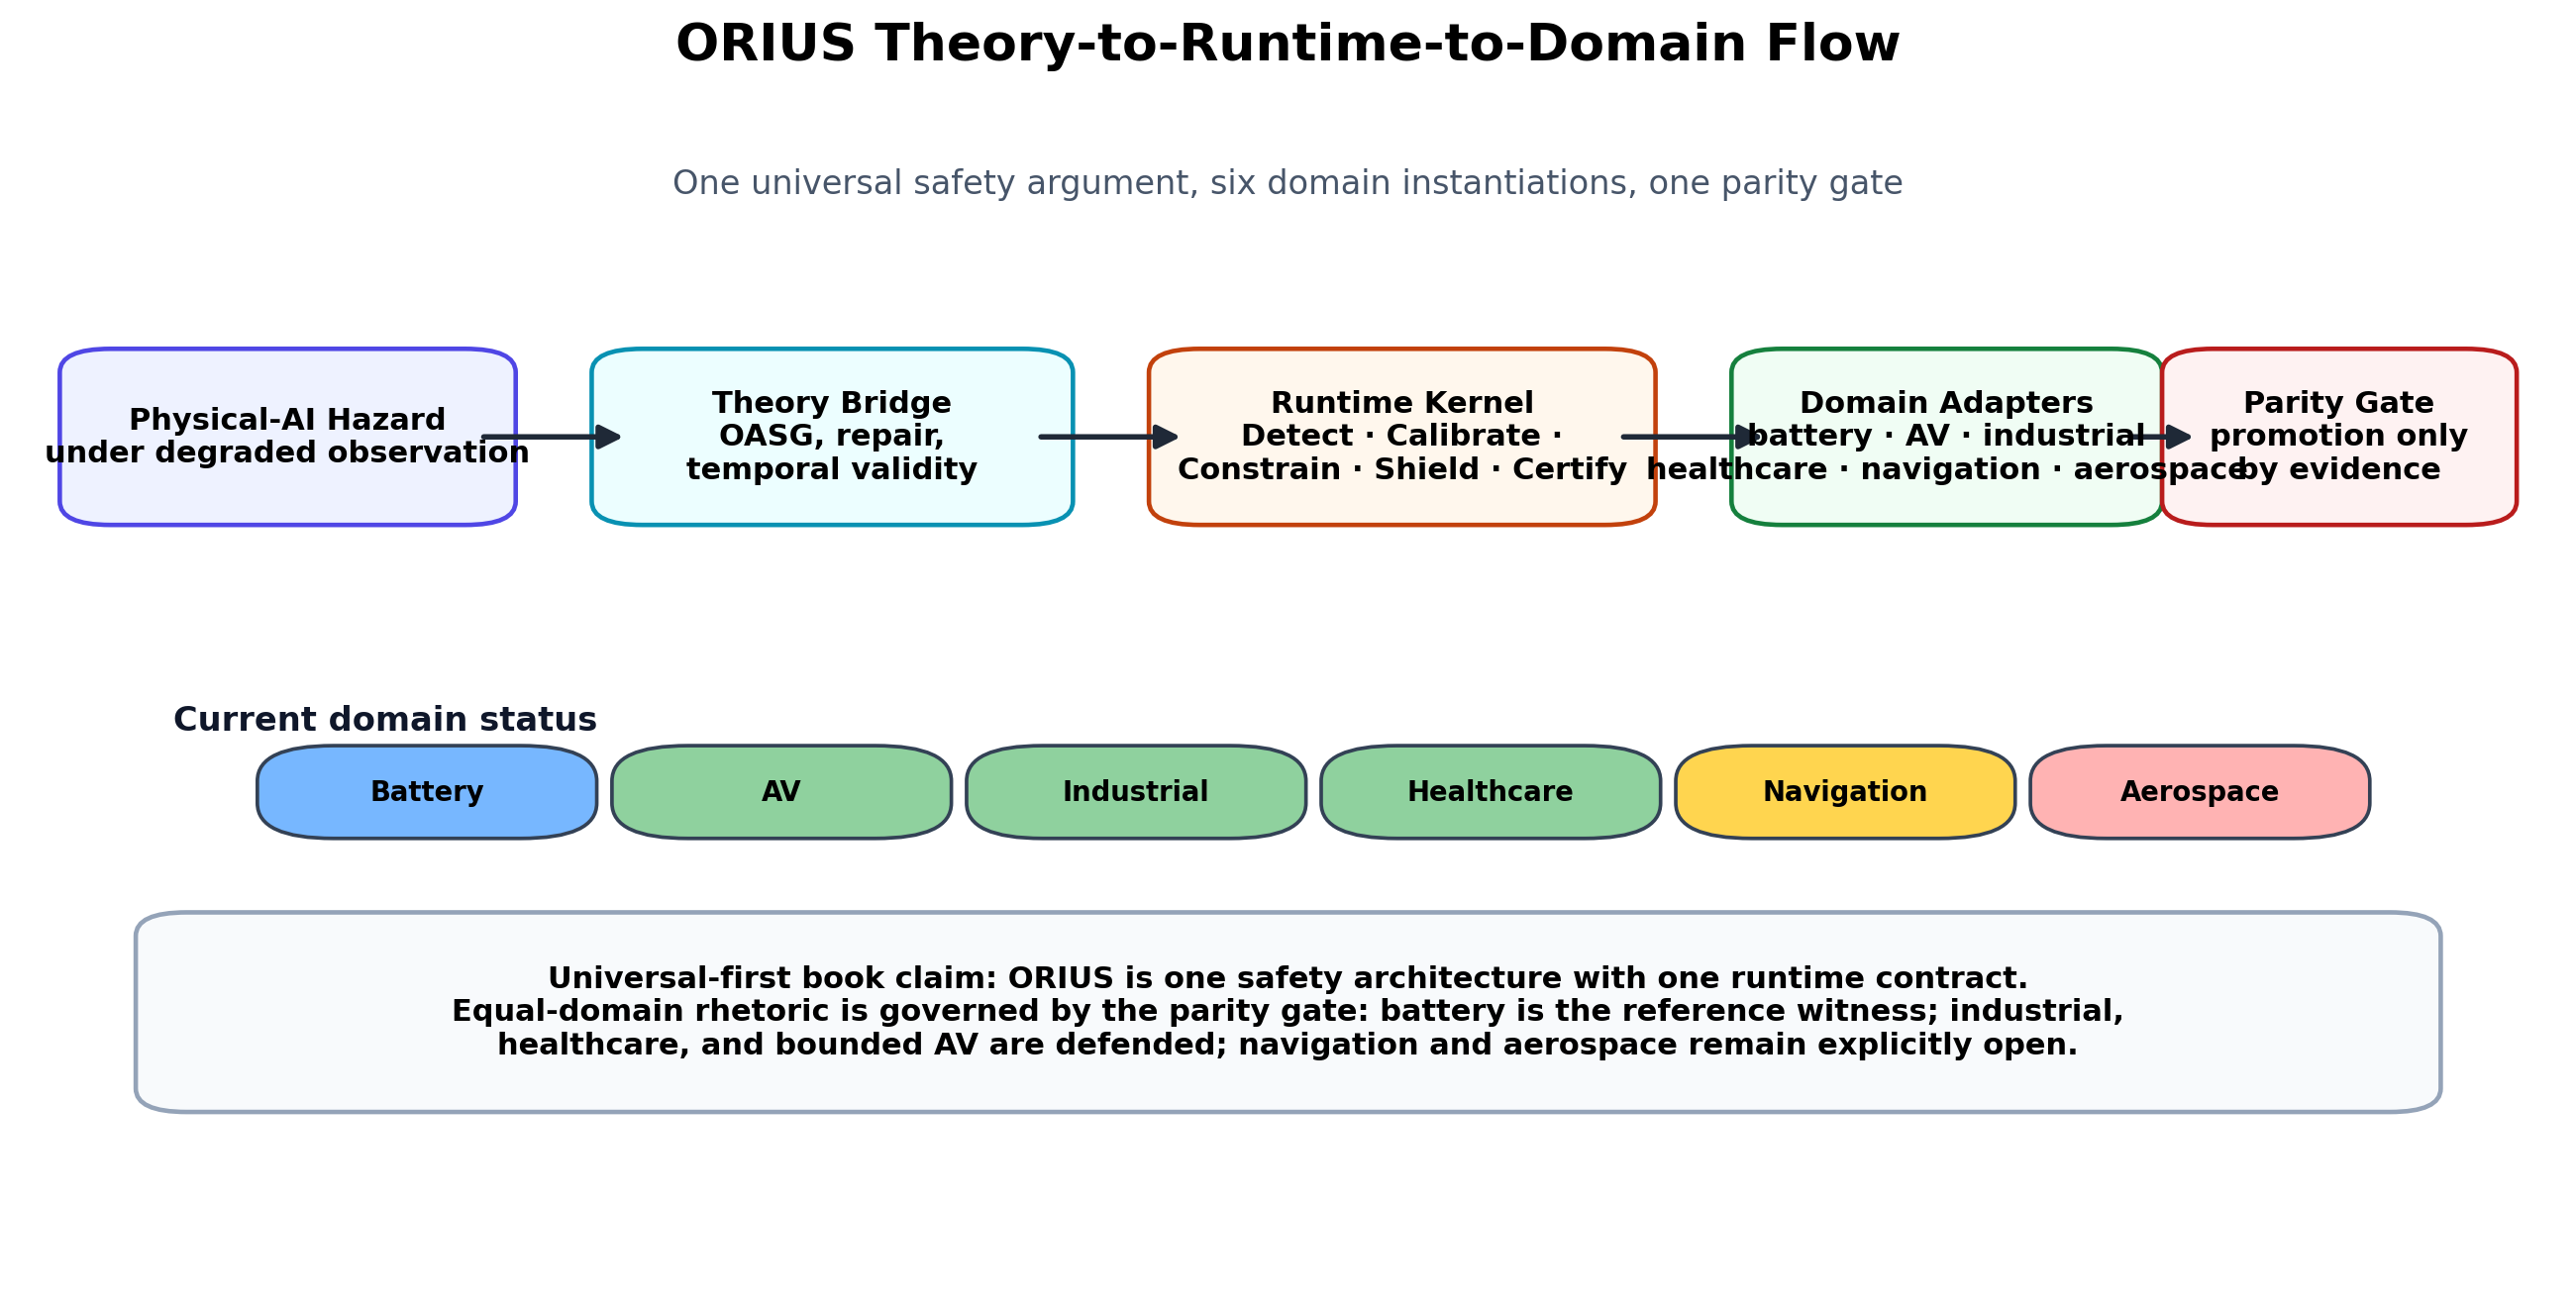
\includegraphics[width=0.94\textwidth]{../reports/publication/fig_orius_theory_runtime_domain_flow.png}%
}
\caption{ORIUS runtime flow from degraded telemetry to repaired action and governed
certificate. The figure is generated from the same publication assets that feed the
manuscript-facing parity and governance surfaces.}
\label{fig:orius-runtime-step}
\end{figure}

Figure~\ref{fig:orius-runtime-step} makes the runtime object concrete. Reliability is not a
dashboard number layered on top of an unchanged controller. It changes the admissible state
set, which changes the admissible action set, which in turn changes whether nominal action
may be released, whether it must be repaired, or whether the runtime must fall back to a
safer policy. Certification closes the loop by recording what was released, why it remained
admissible, and when that justification should expire.

\section{DomainAdapter as the universal boundary}
The \texttt{DomainAdapter} contract is the narrow interface that makes universality
credible. The adapter owns the local semantics that should remain local:
\begin{itemize}
  \item how raw telemetry is interpreted into state features;
  \item how true-state violation and observed-state satisfaction are defined;
  \item how candidate action is repaired or projected;
  \item what fallback means for the plant; and
  \item what certificate payload must be preserved for reviewable release.
\end{itemize}
The universal kernel owns what should remain shared:
\begin{itemize}
  \item reliability handling;
  \item uncertainty inflation;
  \item admissible-set tightening;
  \item benchmark-schema compatibility; and
  \item certificate lifecycle discipline.
\end{itemize}

\IfFileExists{paper/assets/tables/generated/tbl_universal_framework.tex}{%
% ORIUS Universal Domain Physical Safety Framework
% Generated for paper inclusion

% Table 1: Domain State Schema
\begin{table}[t]
\centering
\caption{Domain state schema for ORIUS universal framework.}
\label{tab:universal-state}
\begin{tabularx}{\textwidth}{@{}lXlX@{}}
\toprule
\textbf{Domain} & \textbf{State Fields} & \textbf{Unit} & \textbf{Description} \\
\midrule
Battery & soc\_mwh, load\_mw, renewables\_mw & MWh, MW & Battery SOC and dispatch context \\
AV & ego\_speed\_mps, relative\_gap\_m, ttc & m/s, m, s & Bounded nuPlan longitudinal replay context \\
Healthcare & hr\_bpm, spo2\_pct, respiratory\_rate & bpm, \%, /min & Retrospective monitoring and alert context \\
\bottomrule
\end{tabularx}
\end{table}

% Table 2: Safety Predicates
\begin{table}[t]
\centering
\caption{Safety predicates per domain.}
\label{tab:universal-safety}
\begin{tabularx}{\textwidth}{@{}lXX@{}}
\toprule
\textbf{Domain} & \textbf{Safety Predicate} & \textbf{Config Key} \\
\midrule
Battery & SOC $\in$ [min\_soc, max\_soc]; charge/discharge mutual exclusion & min\_soc\_mwh \\
AV & TTC and predictive-entry barrier remain satisfied on the bounded nuPlan replay state & ttc\_min, gap\_min \\
Healthcare & vital alert release remains inside the bounded monitoring envelope & spo2\_min\_pct, hr\_bounds \\
\bottomrule
\end{tabularx}
\end{table}

% Table 3: Pipeline Stages
\begin{table}[t]
\centering
\caption{Universal DC3S pipeline stages.}
\label{tab:universal-pipeline}
\begin{tabular}{clll}
\toprule
\textbf{Stage} & \textbf{Name} & \textbf{Adapter Method} & \textbf{Output} \\
\midrule
1 & Detect & compute\_oqe & $w_t$, flags \\
2 & Calibrate & build\_uncertainty\_set & $\mathcal{U}_t$, meta \\
3 & Constrain & tighten\_action\_set & $\mathcal{A}_t$ \\
4 & Shield & repair\_action & safe\_action, repair\_meta \\
5 & Certify & emit\_certificate & certificate \\
\bottomrule
\end{tabular}
\end{table}
%
}{%
% ORIUS Universal Domain Physical Safety Framework
% Generated for paper inclusion

% Table 1: Domain State Schema
\begin{table}[t]
\centering
\caption{Domain state schema for ORIUS universal framework.}
\label{tab:universal-state}
\begin{tabularx}{\textwidth}{@{}lXlX@{}}
\toprule
\textbf{Domain} & \textbf{State Fields} & \textbf{Unit} & \textbf{Description} \\
\midrule
Battery & soc\_mwh, load\_mw, renewables\_mw & MWh, MW & Battery SOC and dispatch context \\
AV & ego\_speed\_mps, relative\_gap\_m, ttc & m/s, m, s & Bounded nuPlan longitudinal replay context \\
Healthcare & hr\_bpm, spo2\_pct, respiratory\_rate & bpm, \%, /min & Retrospective monitoring and alert context \\
\bottomrule
\end{tabularx}
\end{table}

% Table 2: Safety Predicates
\begin{table}[t]
\centering
\caption{Safety predicates per domain.}
\label{tab:universal-safety}
\begin{tabularx}{\textwidth}{@{}lXX@{}}
\toprule
\textbf{Domain} & \textbf{Safety Predicate} & \textbf{Config Key} \\
\midrule
Battery & SOC $\in$ [min\_soc, max\_soc]; charge/discharge mutual exclusion & min\_soc\_mwh \\
AV & TTC and predictive-entry barrier remain satisfied on the bounded nuPlan replay state & ttc\_min, gap\_min \\
Healthcare & vital alert release remains inside the bounded monitoring envelope & spo2\_min\_pct, hr\_bounds \\
\bottomrule
\end{tabularx}
\end{table}

% Table 3: Pipeline Stages
\begin{table}[t]
\centering
\caption{Universal DC3S pipeline stages.}
\label{tab:universal-pipeline}
\begin{tabular}{clll}
\toprule
\textbf{Stage} & \textbf{Name} & \textbf{Adapter Method} & \textbf{Output} \\
\midrule
1 & Detect & compute\_oqe & $w_t$, flags \\
2 & Calibrate & build\_uncertainty\_set & $\mathcal{U}_t$, meta \\
3 & Constrain & tighten\_action\_set & $\mathcal{A}_t$ \\
4 & Shield & repair\_action & safe\_action, repair\_meta \\
5 & Certify & emit\_certificate & certificate \\
\bottomrule
\end{tabular}
\end{table}
%
}

This separation is the implementation answer to the universality question. ORIUS does not
argue that every domain shares one plant geometry. It argues that each domain can expose its
own geometry through one runtime contract while the safety logic surrounding degraded
observation remains reusable.

\section{Relationship to supervision and safety filters}
ORIUS should be read as compatible with, not opposed to, established safety-filter and
runtime-assurance ideas. Control barrier functions, predictive safety filters, and robust
MPC show how plant constraints can be translated into admissible control updates
\cite{ames2019control,ames2014cbf,wabersich2021predictive,mayne2005robust}. Simplex-style
runtime assurance shows how a high-performance controller can be supervised by a safer
fallback authority when operating conditions invalidate the nominal control contract
\cite{sha1998simplex,sha2001using}.

ORIUS differs in emphasis. It freezes degraded observation itself as the opening object of
the runtime step. Reliability loss is not merely one more disturbance bound; it is the
mechanism that tells the runtime when the meaning of observed-state legality has changed.
That is why Detect and Calibrate appear before Shield. The runtime does not only ask how to
project action back into a safe set. It asks how the safe set should be redefined once the
observation channel can no longer be trusted at face value.

\section{Certificate emission and operational semantics}
Certify is not bookkeeping. Once repaired action is released, the runtime must still say
what assumptions justified release, which fallback would be taken if the certificate
expired, and how later review can reconstruct the decision. In ORIUS, certificate metadata
therefore sits inside the same runtime object as reliability, repair, and fallback.

This is what turns ORIUS from a controller-side heuristic into a governed runtime layer. The
release record must be causal, bounded, and auditable. That discipline is what makes it
possible to compare domains through runtime artifacts rather than after-the-fact narrative.

\section{Runtime cost and operational realism}
ORIUS is written for operational settings rather than theorem exposition alone. Runtime
overhead, fallback behavior, and auditable certificates are therefore part of the scientific
object. A safety layer that cannot act in time, cannot preserve a coherent lifecycle state,
or cannot explain why it intervened is not a convincing architecture for physical AI.

That operational constraint is what leads naturally into the next two chapters. Once the
runtime layer has been fixed as the central object, the next question is what can actually
be proved about it and how those claims can be measured without confusing nominal coherence
for physical safety.

\section{Architectural takeaway}
What this chapter establishes is architectural rather than empirical closure. ORIUS provides
a reusable runtime contract that translates degraded observation into
reliability-conditioned uncertainty, tightened action legality, repaired or fallback
release, and certificate-aware governance. Stronger claims about optimality, plant realism,
or deployment maturity remain tied to the benchmark rows and governed evidence surfaces that
follow.
